% Created 2024-03-12 Tue 11:38
% Intended LaTeX compiler: pdflatex
\documentclass[a4paper,11pt]{article}
\usepackage[utf8]{inputenc}
\usepackage[T1]{fontenc}
\usepackage{graphicx}
\usepackage{longtable}
\usepackage{wrapfig}
\usepackage{rotating}
\usepackage[normalem]{ulem}
\usepackage{amsmath}
\usepackage{amssymb}
\usepackage{capt-of}
\usepackage{hyperref}
\usepackage[inkscapelatex=false]{svg}
\usepackage[margin=1in]{geometry}
\author{Vijay Panchal}
\date{\today}
\title{Report on AC susceptometer instrumentation}
\hypersetup{
 pdfauthor={Vijay Panchal},
 pdftitle={Report on AC susceptometer instrumentation},
 pdfkeywords={},
 pdfsubject={},
 pdfcreator={Emacs 28.2 (Org mode 9.5.5)}, 
 pdflang={English}}
\begin{document}

\maketitle
Our main goal of the project is to find phase transitions of known materials by looking at its magnetic properties. This mega goal has many obstacles, primarily is noise in final voltage output as our signal is highly feeble. We came across the most logical procedure and took too many points and gave statistics its power. Here, we took some initial data of a known sample to find some constant parameter of our sample we term is some K (kappa). This K will relate between our voltage and magnetic susceptibility for our future purpose. For this we have took three data of known sample,

\begin{enumerate}
\item Fe\textsubscript{2}O\textsubscript{3}
\item Nickel
\item LSMO
\end{enumerate}

\section{some results}
\label{sec:org6b612a1}
These results are down here. Here I plotted Absolute values of voltages i took at random instances, i found a clear trend in values of voltages with and without sample. 

\begin{figure}[!ht]\center
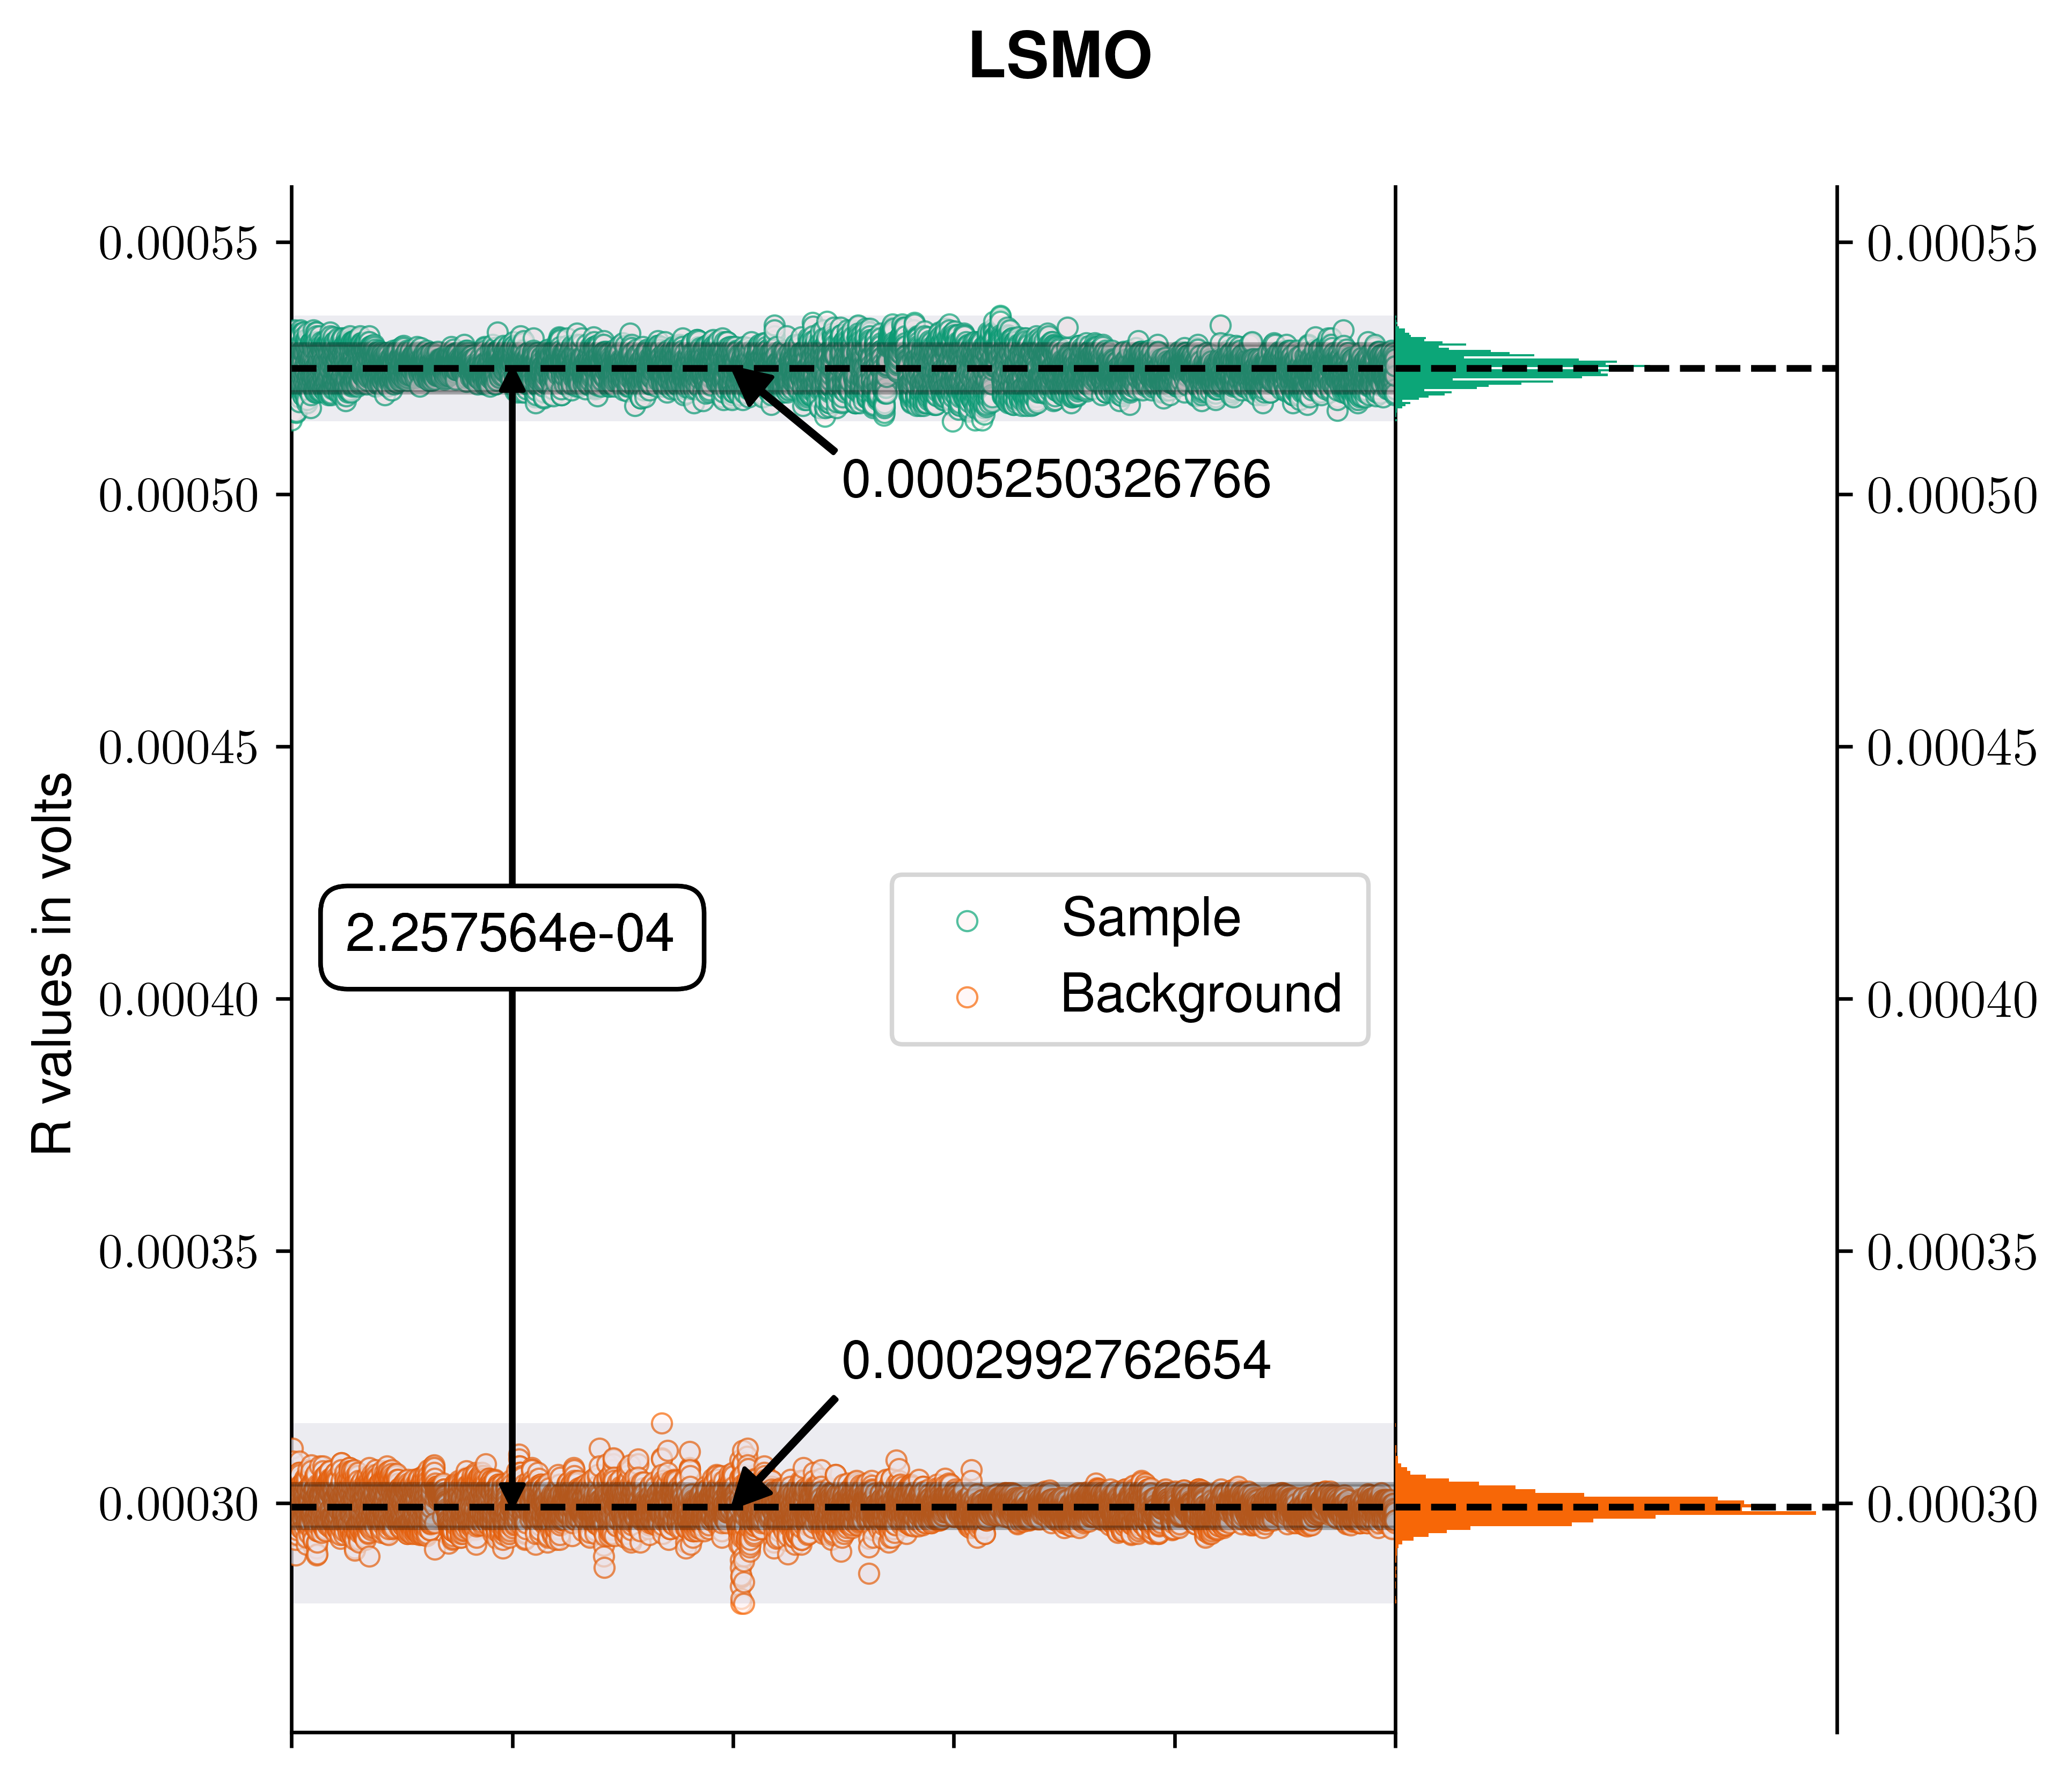
\includegraphics[width=0.7\textwidth]{LSMOR.png}
\caption{This is figure for LSMO absolute voltage levels at random 10000 readings}
\end{figure}


\begin{figure}[hbt!]\center
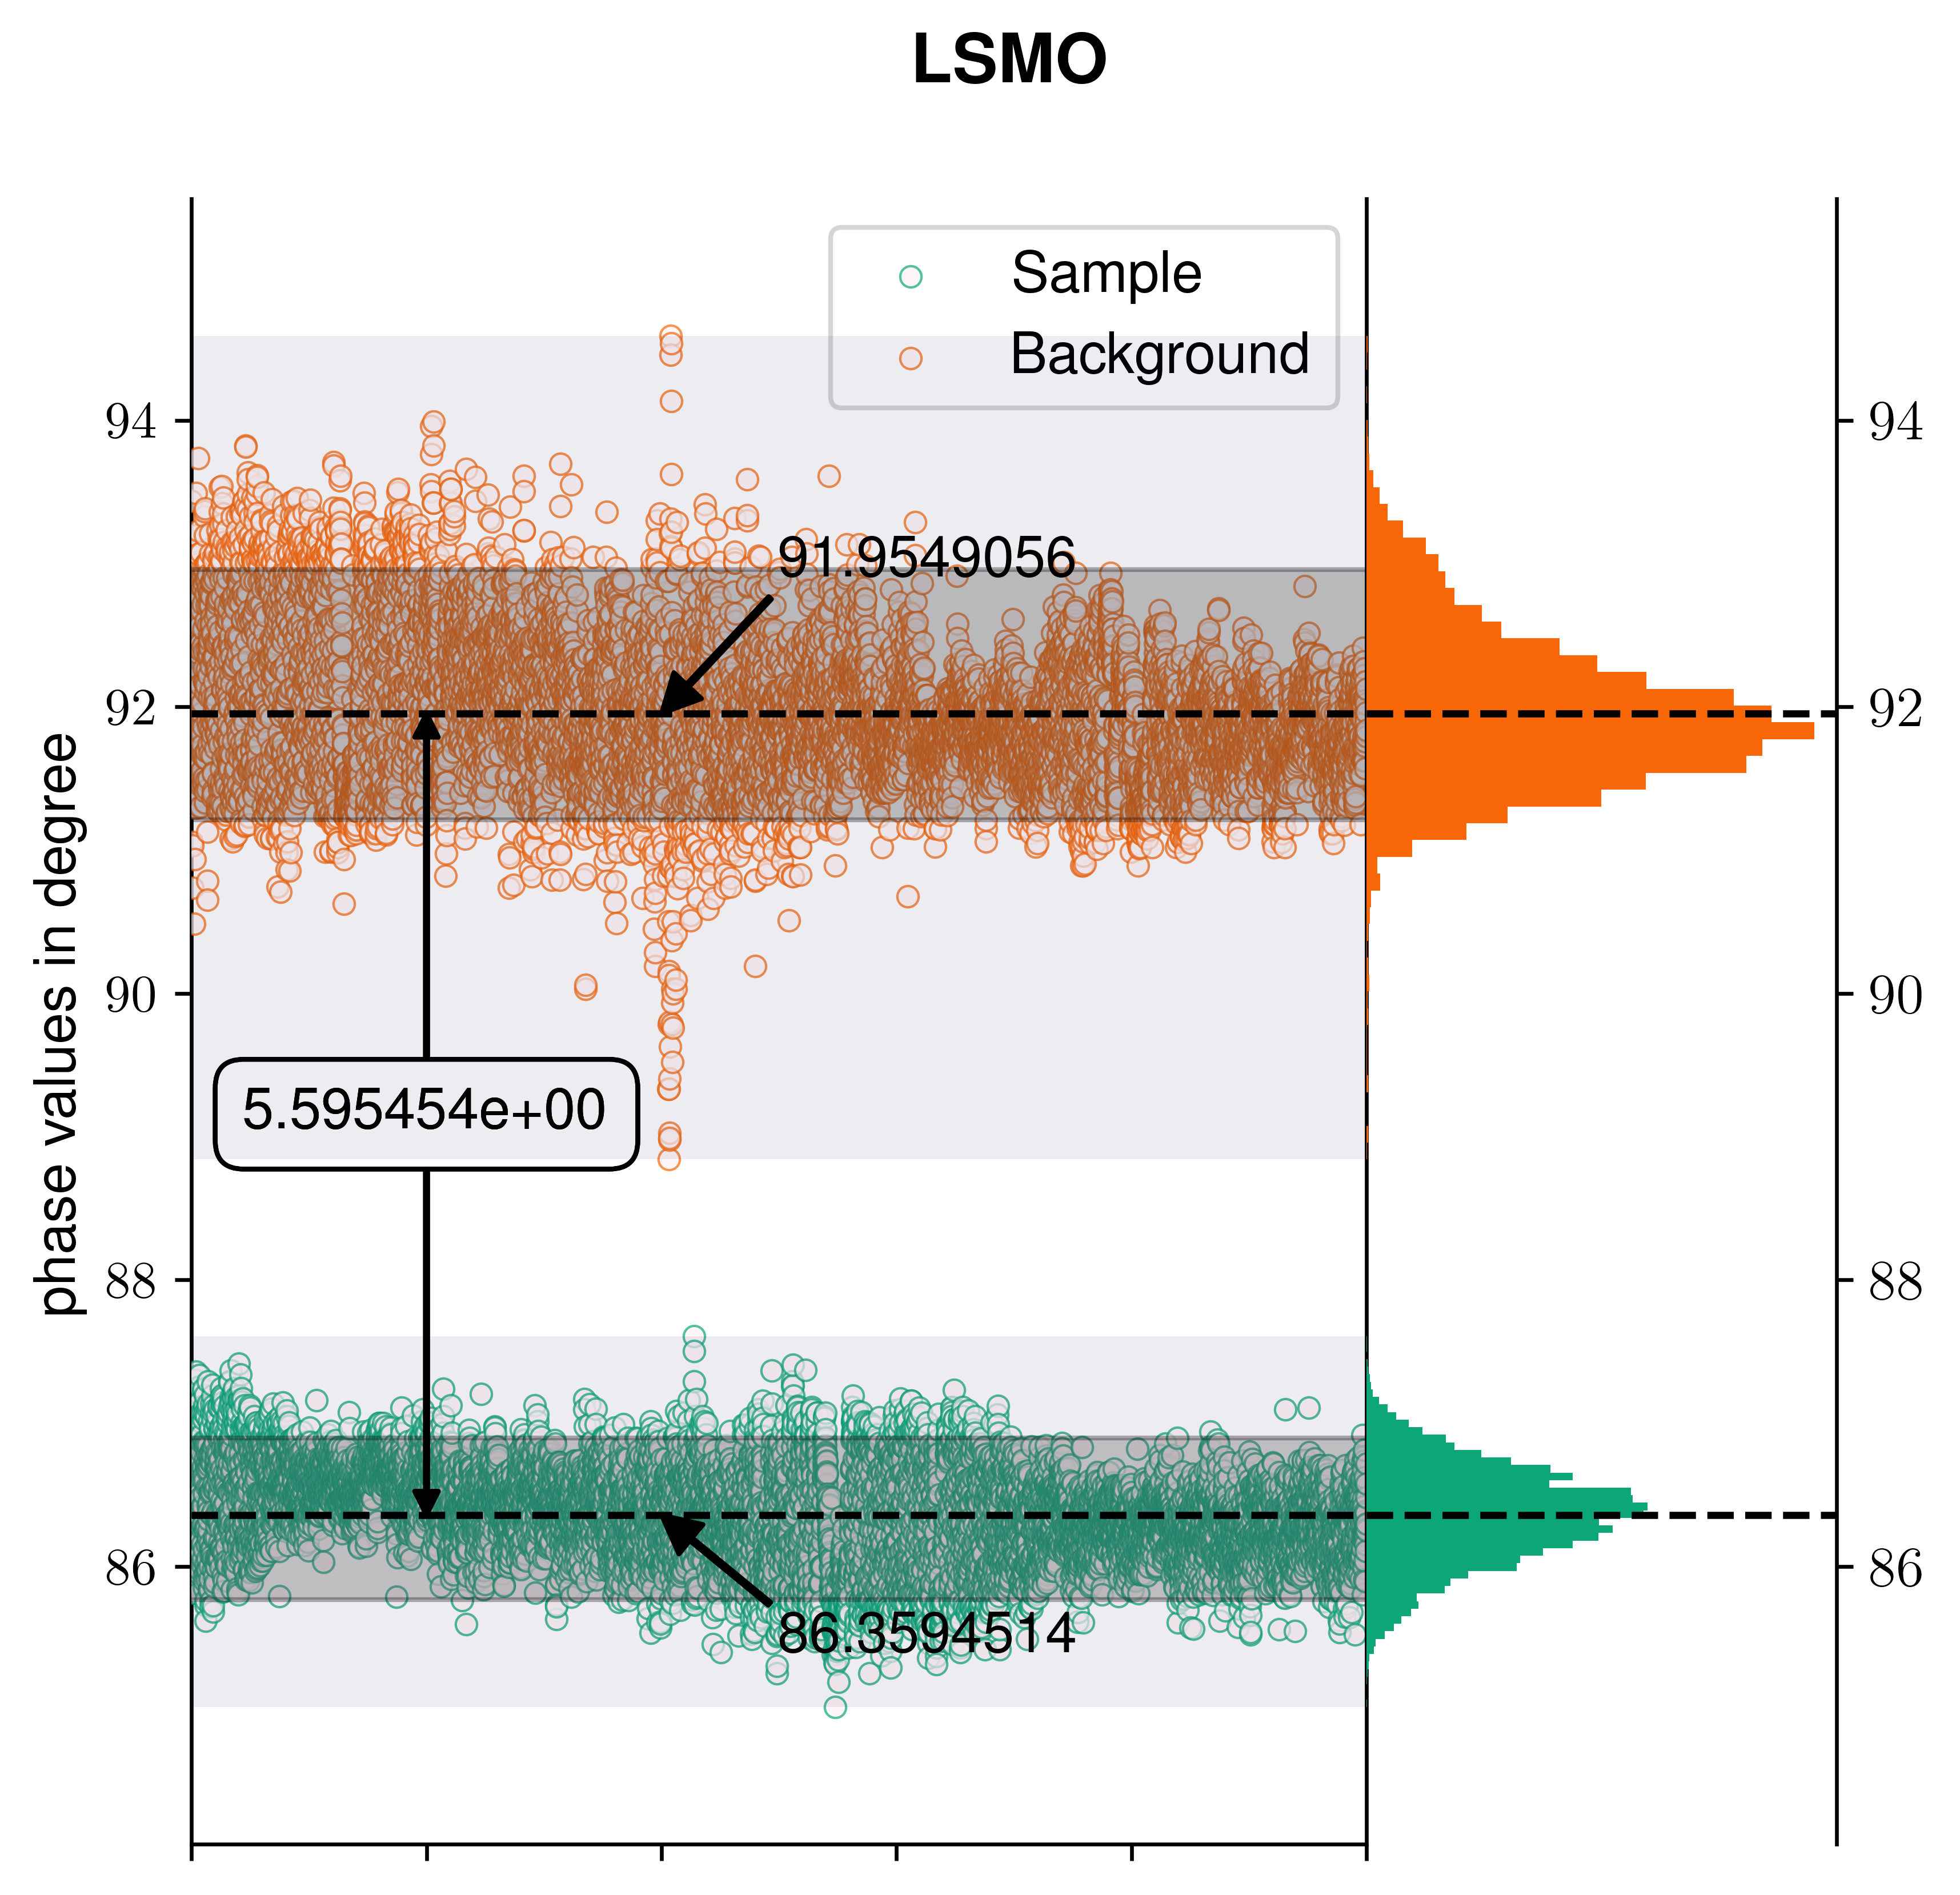
\includegraphics[width=0.7\textwidth]{LSMOT.png}
\caption{This is figure for LSMO phase  readings at random 10000 readings}
\end{figure}

\begin{figure}[!hbt]\center
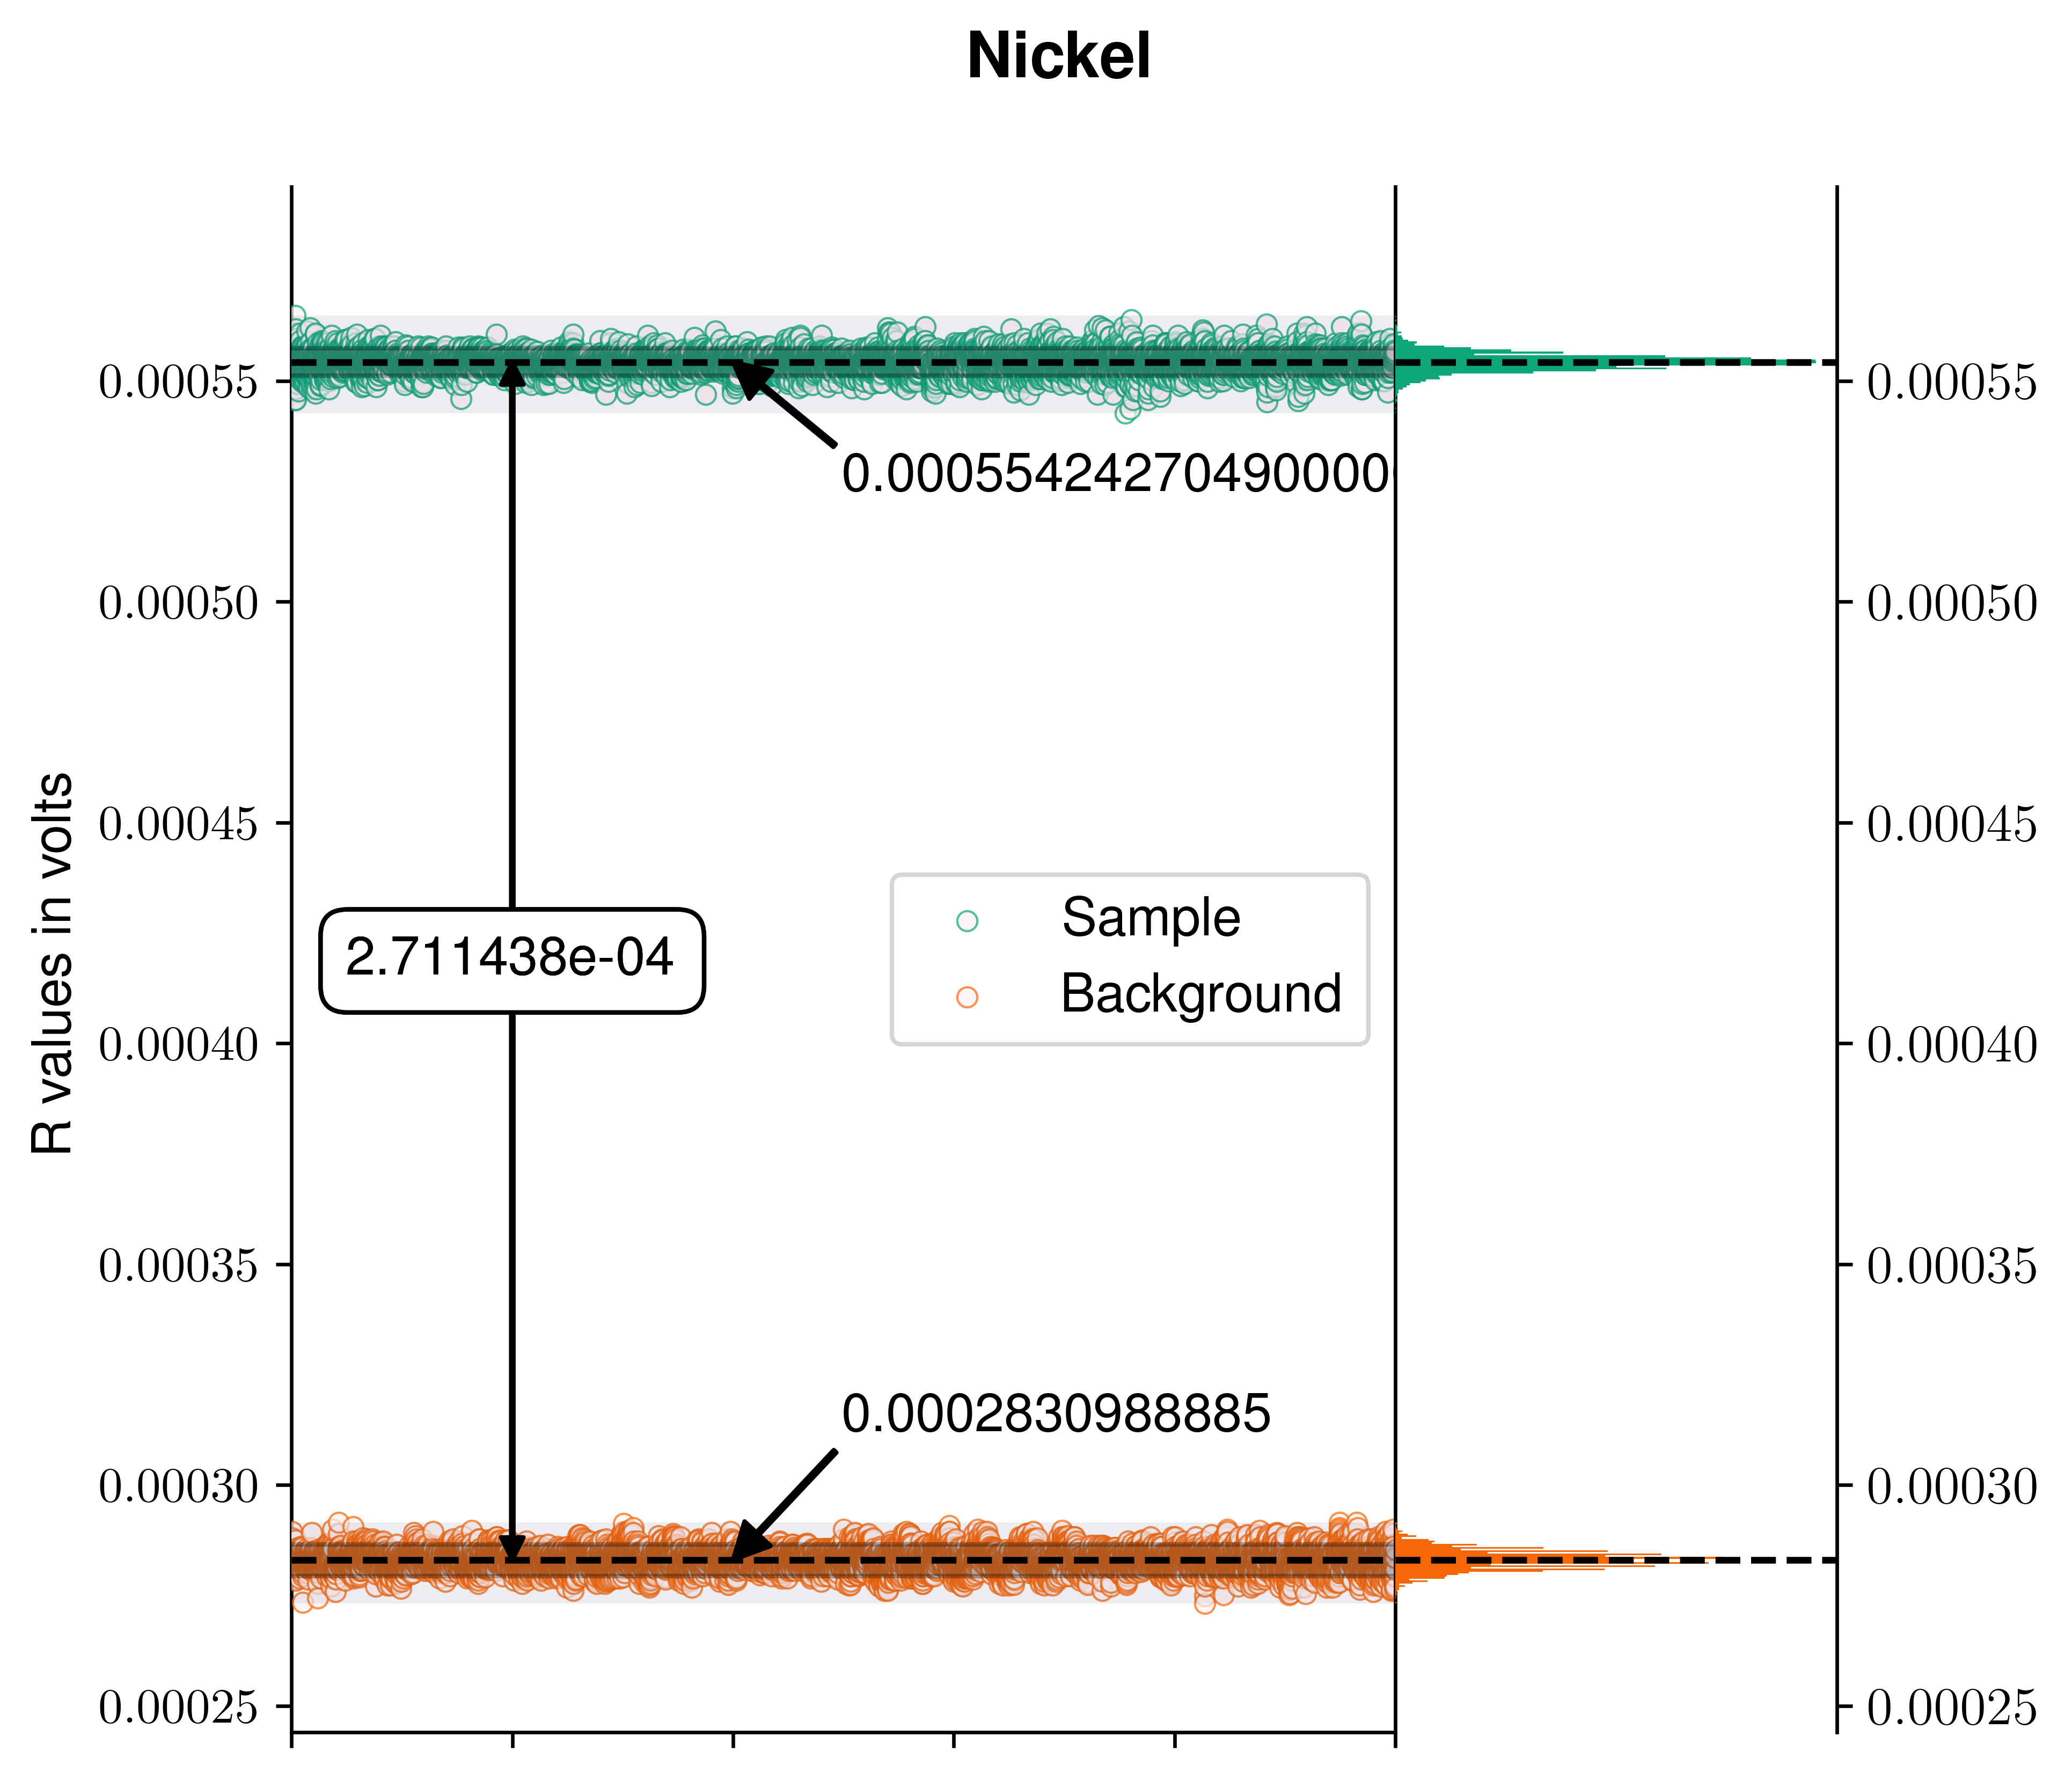
\includegraphics[width=0.7\textwidth]{nickelR.png}
\caption{This is figure for nickel absolute voltage levels at random 10000 readings}
\end{figure}

\begin{figure}[!hbt]\center
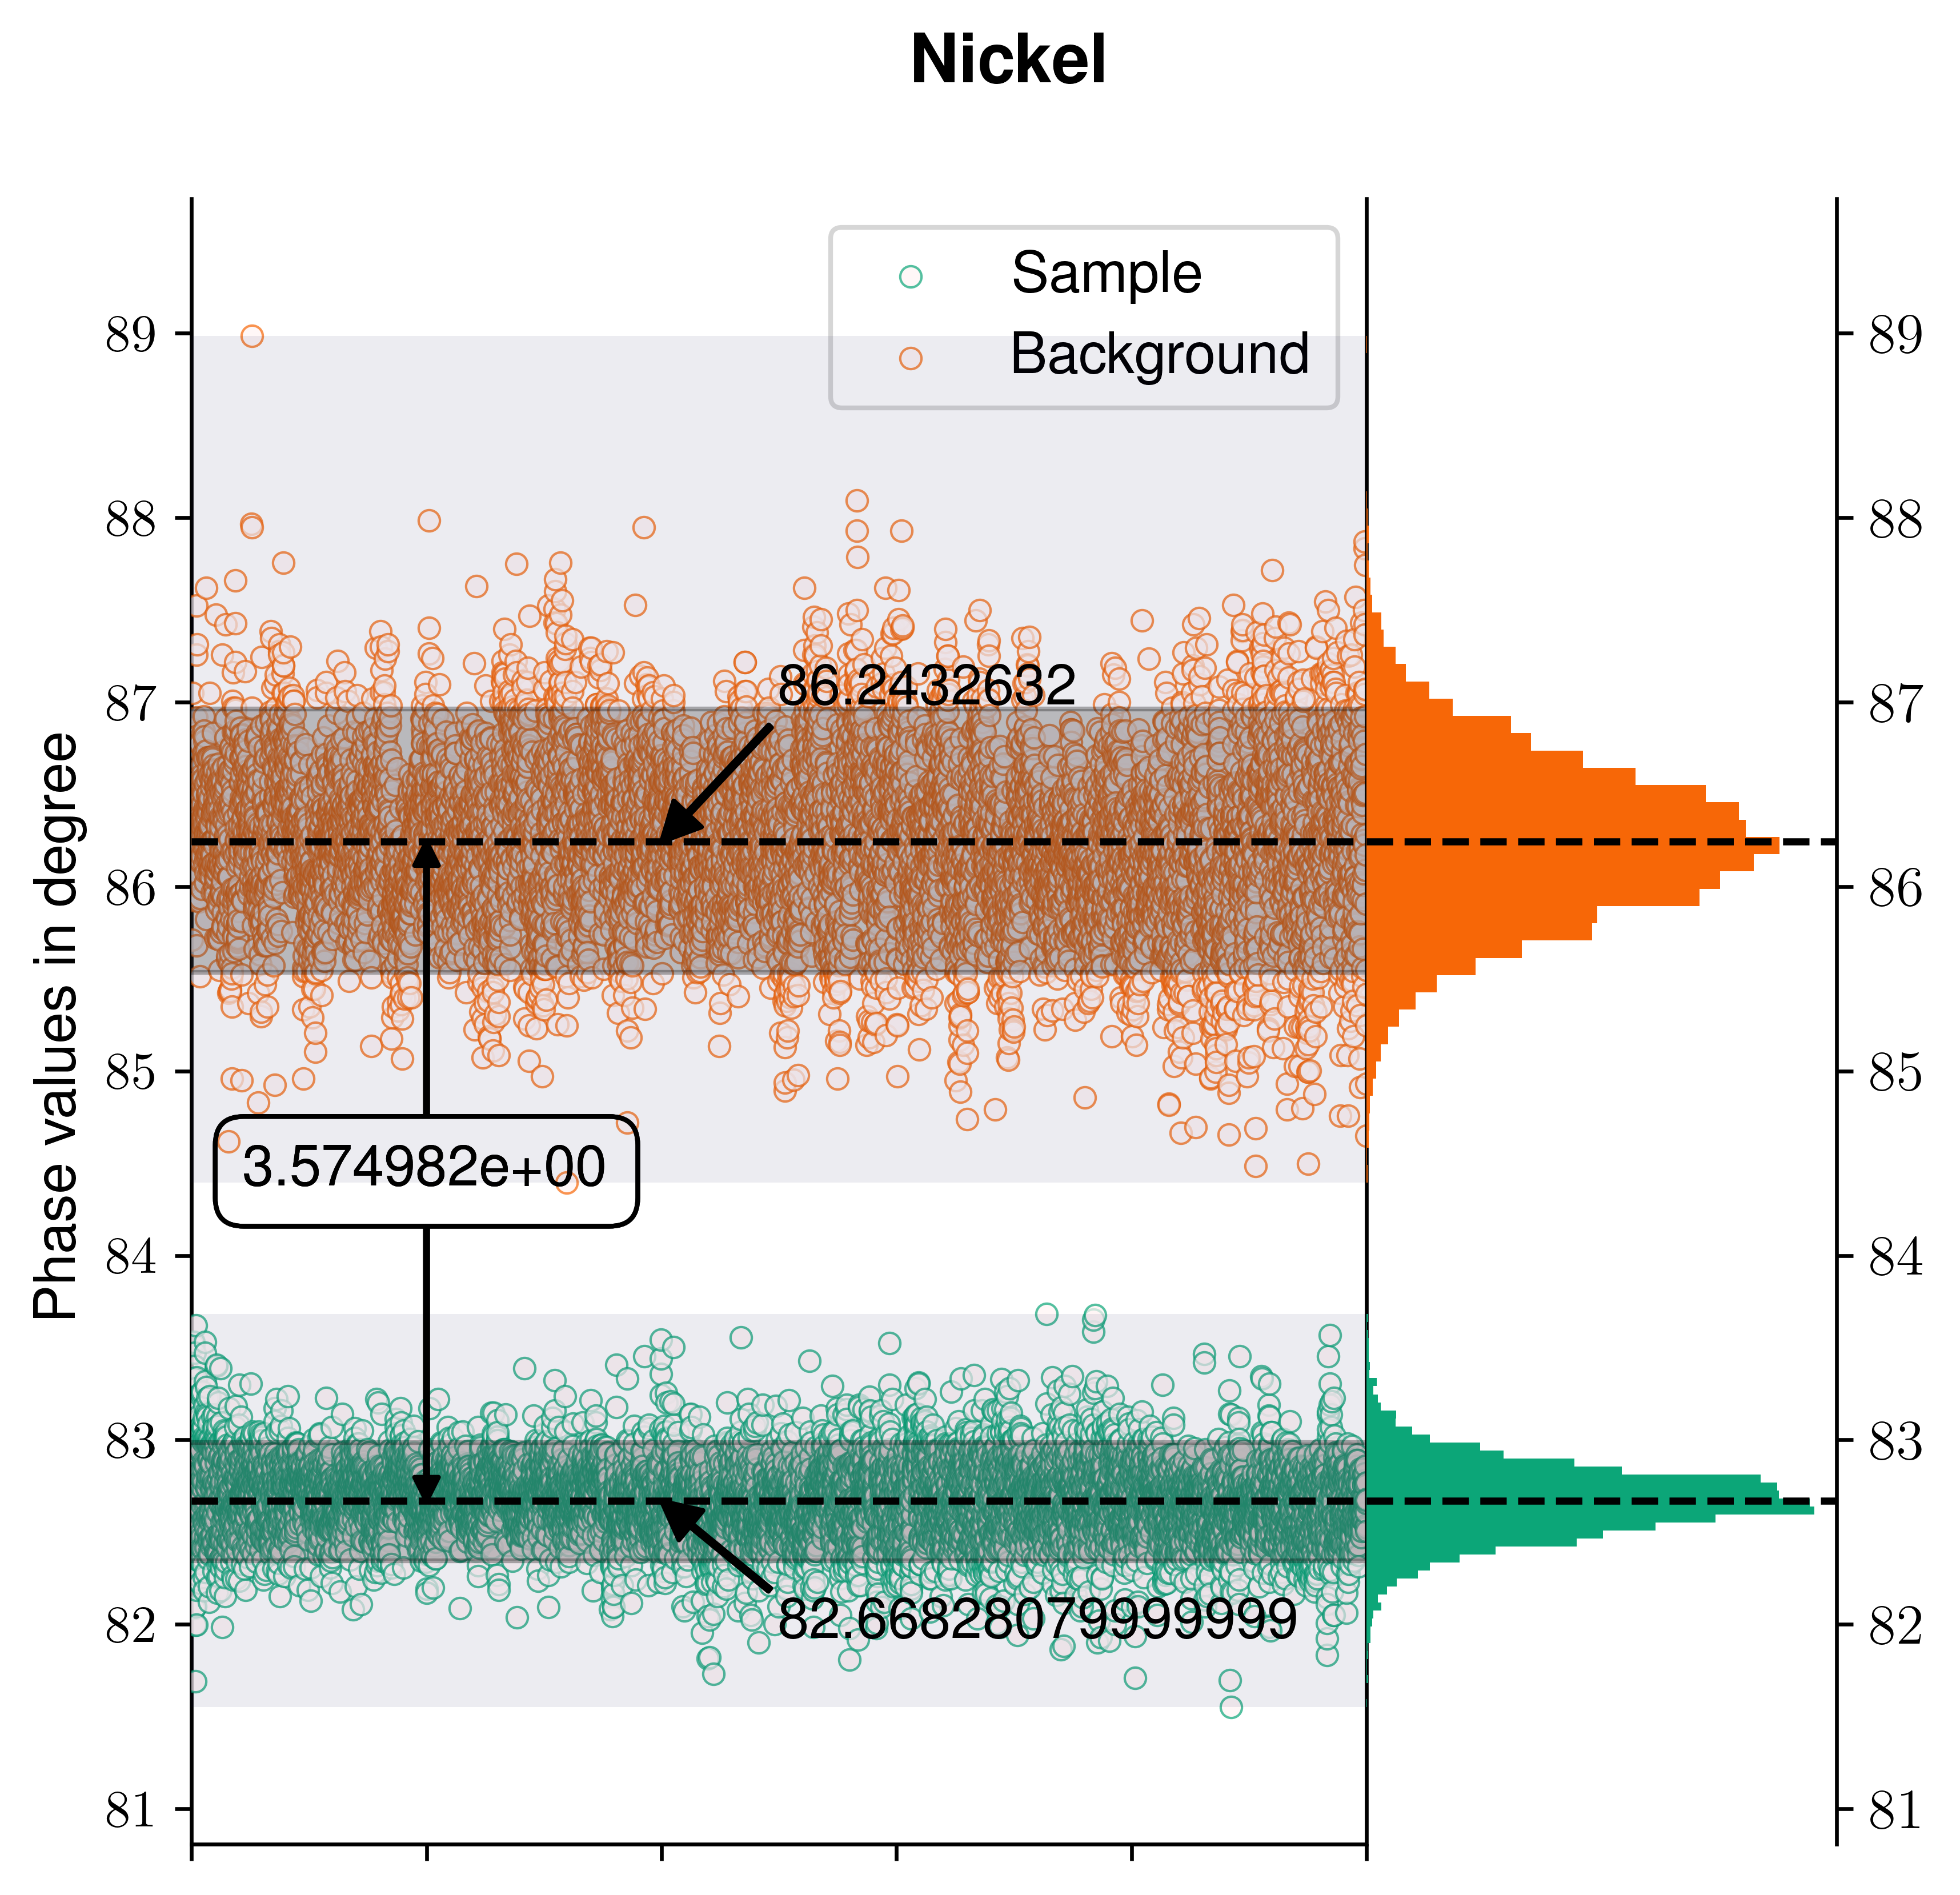
\includegraphics[width=0.7\textwidth]{nickelT.png}
\caption{This is figure for nickel phase at random 10000 readings}
\end{figure}

\clearpage
Second results are from voltage input vs voltage output, here also I found a clear trend.

\begin{figure}[!hbt]\center
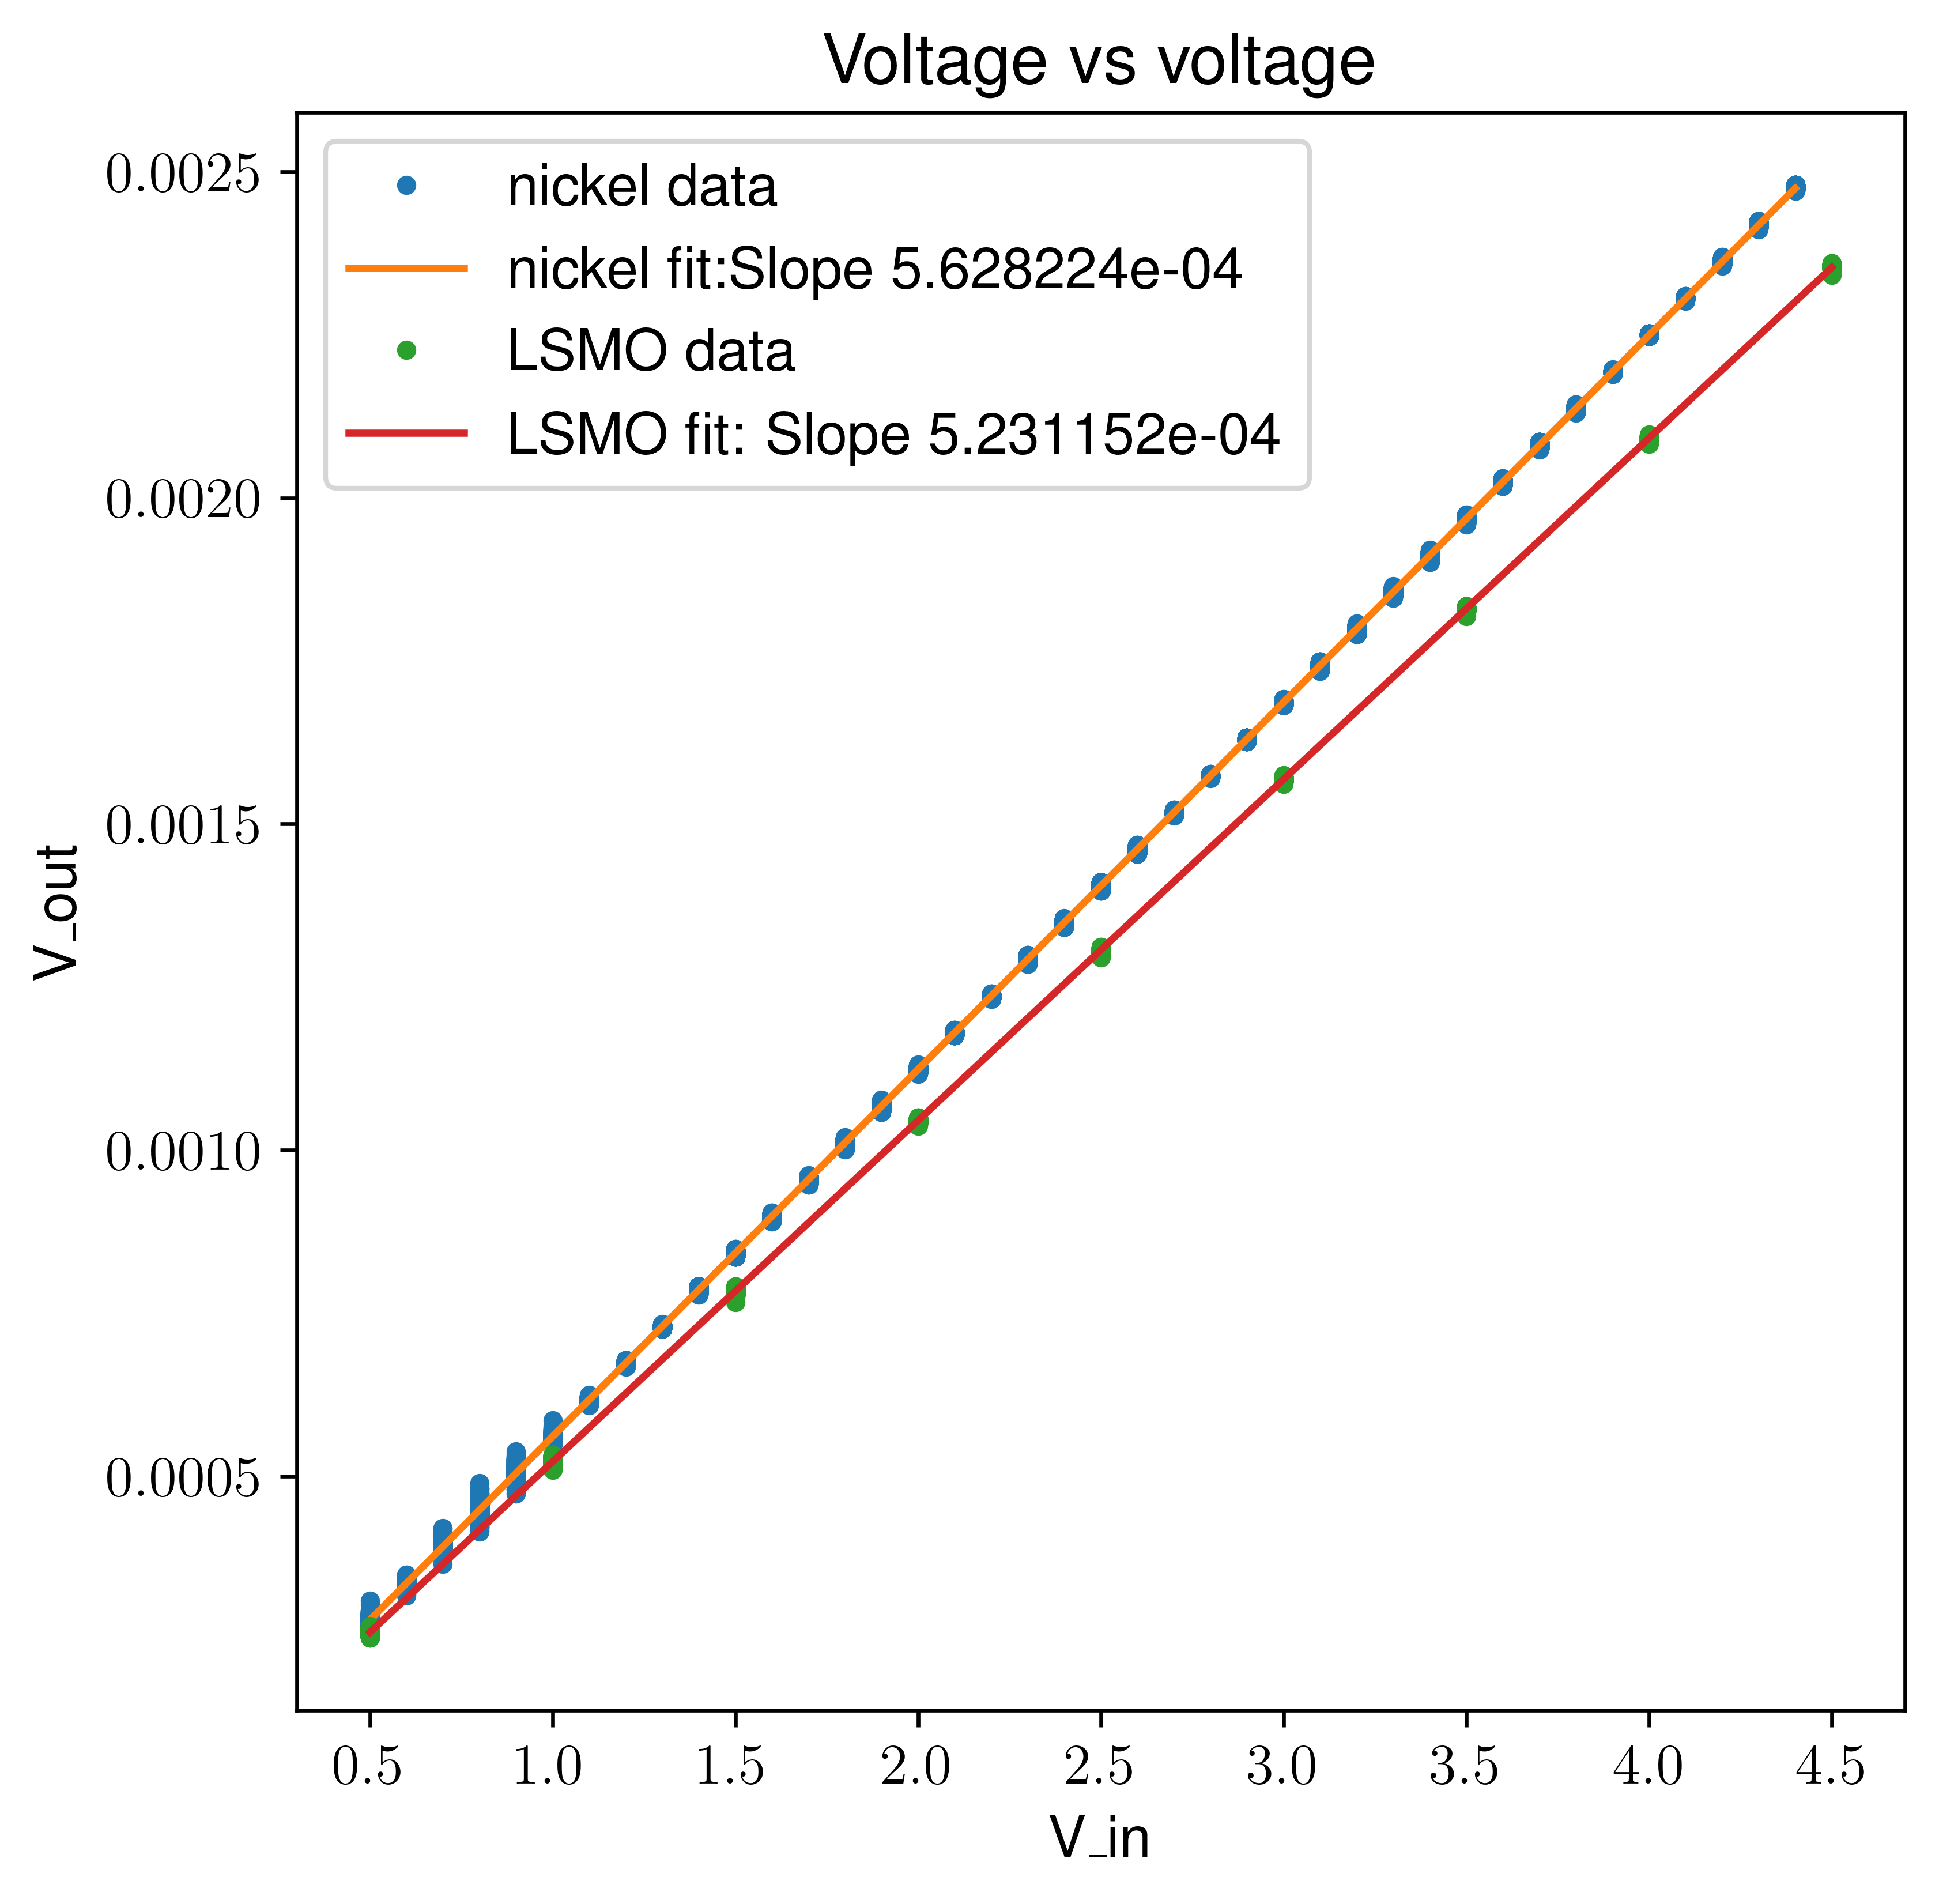
\includegraphics[width=0.7\textwidth]{voltage.png}
\caption{$V_{out}$ vs $V_{in}$ figure for both LSMO and nickel}
\end{figure}


\clearpage

Problems right now, i can’t calibrate the instrument because i don’t know absolute values or approximate good range of AC magnetic susceptibility, and from what range i found i can’t find a reasonable assistant in calibration. 


\section{Some calculations}
\label{sec:org26dd513}

Beginning we thought that voltage and magnetic susceptibility should be related with following realtion ship,

\begin{equation*}
V_{out} \propto \chi
\end{equation*}
\begin{equation*}
V_{out} = K \chi
\end{equation*}
\begin{equation*}
V_{out} = K \frac{\chi^{(sample)} \times W^{(sample)}}{W_{atomic}^{(sample)}}
\end{equation*}

So, our task is find K related to our instrument and calibrate the instrument such that i can find results accurately and related to \(\chi\),

\begin{equation*}
V_{out}^{(LSMO)} = K \chi^{(LSMO)}
\end{equation*}
\begin{equation*}
V_{out}^{(nickel)} = K \chi^{(nickel)}
\end{equation*}

Putting relative values of \(V_{out}\) and \(\chi\) we can approximate our \(K\), this can work as long as our setup is same (that was our hope).

Finally we put our results of \(V_{out}^{(sample)}\) in equations but but we can't find exact values of \(\chi\) for ferro materials which is highly dependent on setup at hand. For LSMO and nickel reading we got following reaults.


\begin{equation*}
2.2575 \times 10^{-4} =  K \frac{\chi^{(LSMO)} \times 0.2}{241.84}
\end{equation*}
here, \(W_{atomic}^{(LSMO)}=226.45\) and \(W^{(LSMO)}=0.2\) 

\begin{equation*}
2.2575 \times 10^{-4} = K \frac{[5 to 10] \times 10^{-5} \times 0.2}{226.45}
\end{equation*}


\begin{equation*}
K \approxeq 2556   to   5116
\end{equation*}

similarly if we take, \(\chi^{(nickel)}= 0.004423\), (\(W_{atomic}^{(nickel)}=58.693\) and \(W^{(nickel)} = 0.1946\))

\begin{equation*}
K \approxeq 18
\end{equation*}


Also, if compare slope of graph then \(\chi^{(nickel)} < \chi{(LSMO)}\), which is hard to believe.
\end{document}